\section{Introduction}
\label{sec:intro}

Agentic on-policy distillation (OPD) trains an agent on its own trajectories. The student acts in a live environment, and a stronger teacher scores every token it produces~\citep{reopd2026}. The teacher never acts in this loop; it only scores, and its next-token distribution on the student's histories is the whole training signal. This form of dense supervision also underlies the multi-teacher post-training pipelines of MiMo-V2-Flash and Nemotron-Cascade 2~\citep{mimo2026,nemotroncascade22026}.

A natural explanation of where agentic OPD goes wrong is compounding error. The student's mistakes carry its trajectories beyond the region where the teacher is reliable, and its scores there are noise. Recent agentic-OPD methods act on this reading and keep training inside the trusted region, by shortening the student's episodes~\citep{tcod2026}, handing turns to the teacher~\citep{guidedopd2026}, replaying teacher prefixes~\citep{reopd2026}, or intervening where the two disagree~\citep{futurebridge2026}, and report gains in their own settings.

We show this explanation is incomplete. We take the states where the untrained student disagrees most with the teacher, late in its episodes, the states that compounding error should place furthest outside the teacher's region, and let the teacher act from them. Its takeovers still finish the task. In every environment they beat the student's own outcome from the same states, and they rescue many of the states the student went on to lose.
The student has not drifted beyond what the teacher can handle. Yet the teacher's plain scores let the student's delay pass: only with one of its finishing takeovers in context do they mark down the student's hedging and searching, and the student trained on the plain scores keeps running out of turns. \Cref{fig:overview} illustrates this.

\begin{figure}[t]
\centering
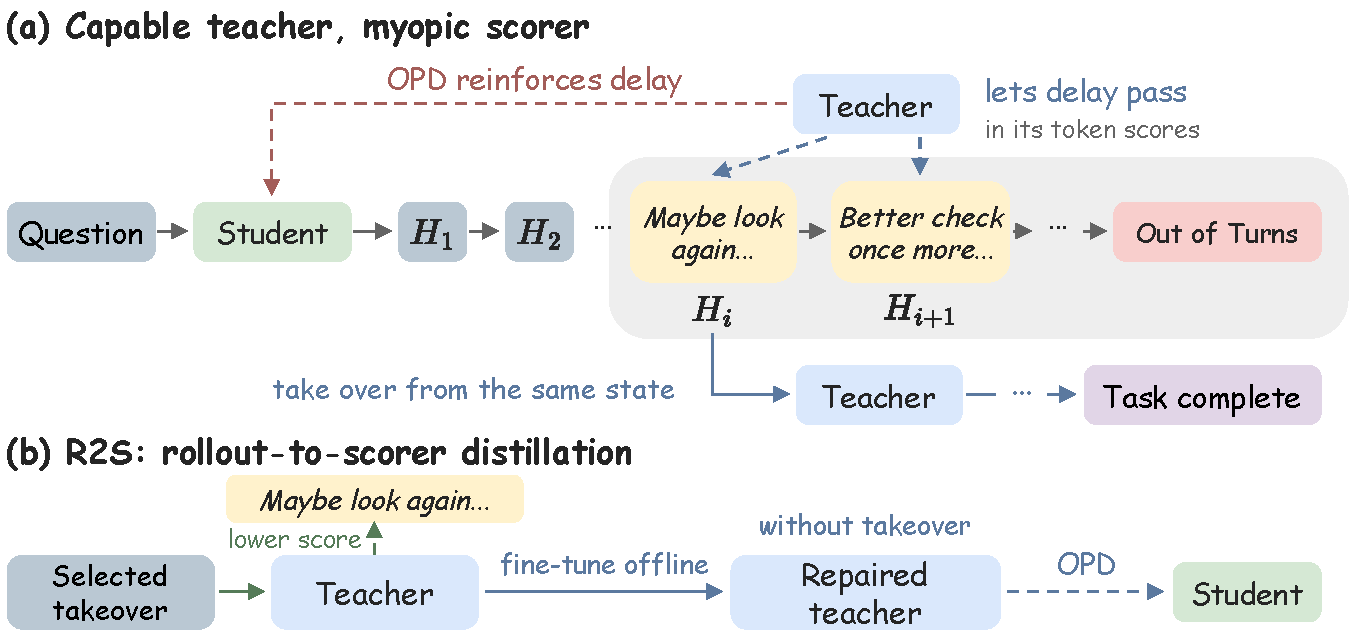
\includegraphics[width=\linewidth]{figures/fig1_teaser.pdf}
\caption{\textbf{OPD can reinforce the delays its teacher lets pass.} (a) The teacher's scores let delaying thoughts pass and the episode runs out of turns; its own takeover from that state finishes. (b) With the takeover in context, the teacher scores the delay lower; \method{} trains a copy to do so without it.}
\label{fig:overview}
\end{figure}


We attribute this to the myopia of next-token scoring. Acting, the teacher writes the whole episode itself: each action is followed by its consequences and by the teacher's own next action, and the episode runs to an outcome. Scoring, it rates each of the student's tokens one at a time, on a history it did not write, without seeing where the episode ends. Under that uncertainty another look or another search keeps options open and is reasonable on its own, so the teacher's scores let it pass. Outcome-based RL punishes such delay with zero reward when the episode runs out, while agentic OPD has no such penalty. We call this difference between what the teacher does and what it scores the \emph{rollout--scorer gap}. This motivates informing the scores with selected teacher continuations.

\methodlong{} (\method{}) repairs the scorer before distillation. First, the teacher takes over from the untrained student's highest-disagreement states. Second, we keep the states where enough takeovers pass a reward-free check, consensus among them or an LLM judge, and pick the shortest passing one as the reference. Third, we fine-tune the teacher to give its takeover-informed scores on every assistant token from the selected divergence turn onward, without the takeover in context. The repaired teacher is frozen for standard OPD. Student training retains the ordinary OPD objective and rollout recipe, and no task reward enters repair or training. We evaluate \method{} across three environments, two teachers and four students under a fixed final-checkpoint protocol. \method{} outperforms three state-of-the-art agentic-OPD methods in every cell. The gain over the best of them in each cell averages $+17.0$ points from the 9B teacher and $+8.5$ from the 30B-A3B teacher.

Our contributions are:
(1) \textbf{The rollout--scorer gap.} \Cref{sec:gap} shows that the teacher's takeovers still finish from the states where the student departs most from it, while its plain scores let the student's delay pass; only a finishing takeover in context turns them against it.
(2) \textbf{\method{}.} \Cref{sec:method} introduces a reward-free repair that moves the teacher's rollout competence into the scores OPD consumes, then freezes the teacher for standard OPD.
(3) \textbf{Evaluation.} We evaluate \method{} against three state-of-the-art agentic-OPD methods across twelve model--environment cells under a shared protocol, and measure target fidelity, out-of-turn rates and searching turns in a long-horizon analysis.
